\chapter{Interfaz de usuario}
\section{Motivación\label{justifUI}}
Antes de comenzar con la planificación, debe ponerse en valor la conveniencia
de esta interfaz de usuario. El principal motivo es que lo que se busca
con este proyecto es crear un producto real, y como tal, no podemos valernos
de un simple lector de puerto serie para el dispositivo, como podría ser
el integrado en el \textit{Arduino IDE}. Además, esta interfaz no solo está
creada con la funcionalidad de este proyecto en mente de servir de mediador
con el usuario para la lectura de las letras escritas con el \textit{SmartPen},
sino que busca ser el nexo de unión de todas las funcionalidades que se
implementen para este. Durante el propio desarrollo de esta interfaz, se
ha reflexionado sobre ciertas funcionalidades, como la de un modo pizarra
donde reflejar el trazado íntegro que se realice, y que se ha propuesto
finalmente como una meta secundaria.

\section{Planificación}
En esta sección se recogerán los motivos por los que se necesita de esta interfaz
de usuario, la elección de herramientas para su desarrollo y el bocetado de la distribución
de sus elementos.

\subsection{Elección de framework para interfaz gráfica}
Las alternativas con las que vamos a partir, tras una fase de documentación sobre
frameworks para desarrollo de interfaces gráficas, preferiblemente multiplataforma,
y sumarlas a las que ya conocía; se recogen en la Figura \ref{tabUI} junto a la valoración
de algunas características importantes.
\begin{table}[h]
    \color{mitexto}
    \begin{tabular}{|l|c|c|c|c|c|c|}
    \hline
    \rowcolor[HTML]{6C737E} 
    \cellcolor[HTML]{6C737E}{\color[HTML]{EFEFEF} \rotatebox{291}{\textbf{Alternativas}}} & \cellcolor[HTML]{6C737E}{\color[HTML]{EFEFEF} \rotatebox{291}{\textbf{Documentación}}} & {\color[HTML]{EFEFEF} \rotatebox{291}{\textbf{Usada anteriormente}}} & {\color[HTML]{EFEFEF} \rotatebox{291}{\textbf{Comunidad}}} & {\color[HTML]{EFEFEF} \rotatebox{291}{\textbf{Soporte para BLE}}} & {\color[HTML]{EFEFEF} \rotatebox{291}{\textbf{Lectura P.Serie nativa~}}} & {\color[HTML]{EFEFEF} \rotatebox{291}{\textbf{Multiplataforma}}} \\ \hline
    \rowcolor[HTML]{C3D6DC} 
    Flutter                                                              & {\color[HTML]{4CDE4C} \cmark}                                               & {\color[HTML]{4CDE4C} \cmark}                                                     & {\color[HTML]{4CDE4C} \cmark}                                           & {\color[HTML]{4CDE4C} \cmark}                                                  & {\color[HTML]{4CDE4C} \cmark}                                                        & {\color[HTML]{4CDE4C} \cmark}                                                 \\
    \rowcolor[HTML]{E8ECF1} 
    GTK+                                                                 & {\color[HTML]{4CDE4C} \cmark}                                               & {\color[HTML]{9B9B9B} -}                                                                         & {\color[HTML]{4CDE4C} \cmark}                                           & {\color[HTML]{FD6864} \xmark}                                                  & {\color[HTML]{FD6864} \xmark}                                         & {\color[HTML]{4CDE4C} \cmark}                                                 \\
    \rowcolor[HTML]{C3D6DC} 
    QT                                                                   & {\color[HTML]{4CDE4C} \cmark}                                               & {\color[HTML]{4CDE4C} \cmark}                                                     & {\color[HTML]{4CDE4C} \cmark}                                           & {\color[HTML]{4CDE4C} \cmark}                                                  & {\color[HTML]{4CDE4C} \cmark}                                                        & {\color[HTML]{4CDE4C} \cmark}                                                 \\
    \rowcolor[HTML]{E8ECF1} 
    PyQT                                                                 & {\color[HTML]{4CDE4C} \cmark}                                               & {\color[HTML]{FD6864} \xmark}                                                     & {\color[HTML]{4CDE4C} \cmark}                                           & {\color[HTML]{4CDE4C} \cmark}                                                  & {\color[HTML]{4CDE4C} \cmark}                                                        & {\color[HTML]{4CDE4C} \cmark}                                                 \\
    \rowcolor[HTML]{C3D6DC} 
    Electron                                                             & {\color[HTML]{4CDE4C} \cmark}                                               & {\color[HTML]{FD6864} \xmark}                                                     & {\color[HTML]{4CDE4C} \cmark}                                           & {\color[HTML]{FD6864} \xmark}                                                  & {\color[HTML]{4CDE4C} \cmark}                                                        & {\color[HTML]{4CDE4C} \cmark}                                                 \\ \hline
    \end{tabular}
    \caption{Tabla de elección de \textit{frameworks} para desarrollo de \textit{UI}s\label{tabUI}}
\end{table}

\textit{Electron} y \textit{GTK} quedan descartados porque, si bien existen
procedimientos para poder gestionar \textit{Bluetooth Low Energy} con estos, no tienen
soporte nativo ni librerías para ello, por tanto, teniendo la posibilidad
de hacer uso de otros frameworks que faciliten esta tarea, es factible
descartar estas opciones.

Ante \textit{QT (C++)} y \textit{PyQT}, debido a que se ha trabajado anteriormente
con \textit{QT (C++)} y el tiempo de desarrollo disponible es un factor
limitante, es razonable excluir \textit{PyQT}.

Solo quedarían \textit{QT} y \textit{Flutter}, se ha escogido ante estas dos
posibilidades \textit{QT}
por dos razones. La primera razón es que \textit{Flutter} está más dirigido
a interfaces móviles. Y la segunda razón es que pese a haber trabajado con
ambas, a título personal, me encuentro más habituado a \textit{QT}.

Por lo que el framework seleccionado para realizar la interfaz de usuario,
será \textit{QT} ya que ofrece soporte para las tecnologías que en principio
van a utilizarse y porque es una herramienta con la que ya se ha trabajado
y esto resulta en un menor tiempo de documentación, causa de peso
por el tiempo tan ajustado.

\subsection{Diseño de la interfaz\label{diseUI}}
Para el bocetado de la interfaz previo a la implementación, se hará uso
de \textit{QT Design Studio}, herramienta de \textit{QT} para diseñar
interfaces.
En el bocetado de la interfaz se fijarán los elementos que la formarán
y su disposición procediendo razonadamente.
Para entender visualmente lo que se va a describir, puede examinar el \textit{apéndice
\ref{ifazUsu}}.


Como se ha razonado en la
Sección \ref{justifUI} anterior, queremos que este programa sea el
\textit{hub} de funcionalidades para el \textit{SmartPen}, por lo que
se hará uso de una barra lateral para acceder a estas. Queremos que
el protagonismo se encuentre en la funcionalidad, por lo que esta
barra lateral será desplegable, para reducir el tamaño que esta ocupe
en la interfaz. Alojará las funcionalidades y, dada la naturaleza académica
del proyecto, una sección sobre el desarrollador, para más información sobre
el trabajo.

Cada sección de la interfaz, se
mostrará en la pantalla central, quedando las barras superior y lateral,
constantemente a la vista ya que la barra lateral sirve para acceder
a otras secciones de la interfaz y la barra superior muestra información
vital.

Es necesario un indicador de conexión y un botón de conexión inalámbrica,
que se ubicarán a la derecha en la barra superior para evitar sobrecargar
la zona izquierda de la interfaz.

En los primeros bocetos se evidenciaba un vacío en la parte central de
la barra superior y también se echaba en falta saber qué pantalla se estaba
mostrando en cada momento, por lo que uniendo ambas carencias, se
solventó disponiendo un indicador de pantalla en dicha región. 

\section{Implementación\label{implemUI}}
En cuanto a la implementación software, al margen de aplicar el diseño
descrito en la Sección \ref{diseUI} anterior, los retos planteados
son principalmente dos.
El primero de ellos: la gestión simultánea de la lógica de la interfaz, la lectura
del puerto serie y la lectura de \textit{características} del servicio
\textit{Bluetooth Low Energy} (definido en la Sección \ref{servBLE}).
El segundo: la implementación de lectura, especialmente la lectura haciendo
uso del servicio \textit{Bluetooth}.

Para afrontarlos, se hará uso de tecnologías que nos proporciona el propio
\textit{framework}. Para gestionar simultáneamente varios procesos, es
posible hacer uso de \textit{hilos} (o \textit{threads}) gracias a los
\textit{QThread}s de \textit{QT}, que proveen de una clase para gestionar
\textit{hilos} independientemente del sistema. Por lo que crearemos un
hilo concurrente a la ejecución de la lógica de la interfaz, que se hará
cargo de los procedimientos de lectura, tanto \textit{Bluetooth} como del
puerto serie; la clase
\href{https://github.com/AntonioPriego/SmartPen/blob/main/SmartPenUI/readerthread.cpp}{\textit{ReaderThread}}.

Por otro lado, para resolver el problema de la lectura de la placa,
tanto la lectura por cable como la inalámbrica, se emplearán
librerías que asisten para estas tareas. Ya se planteó como requisito
que el \textit{framework} de creación de la interfaz, contara con
soporte para las comunicaciones \textit{Bluetooth} y
\textit{puerto serie}. Estas librerías son \textit{QLowEnergy*} y
\textit{QBluetooth*}, y \textit{QSerialPort*} y son parte de las dependencias
que hay que añadir al proyecto.

El resultado de todo lo implementado será lo que refleja la Figura \ref{diagFlujoQT}.

\section{Traspaso del diseño a \textit{QT creator}\label{trasaQT}}
Siguiendo el esquema de diseño de la Sección \ref{diseUI} (\textit{Diseño de la interfaz})
y gracias a la herramienta \textit{Design} de \textit{QT creator},
el traspaso es trivial; crear la estructura, añadir botones, widgets
y demás elementos de la interfaz. Con estos dispuestos, ya es posible
comenzar a trabajar con la lógica detrás estos y su configuración.

Para ver el resultado obtenido, consulte el apéndice \ref{ifazUsu}.

\section{Configuración de la interfaz}
La configuración de la interfaz consistirá en inicializar los parámetros
con los que parten los elementos creados en la Sección \ref{trasaQT} anterior
y definir su comportamiento durante la ejecución.

Para el acceso a cada sección, se plantea un widget que varía su
contenido en función del índice seleccionado.
De esta forma se guarda el resto de la interfaz inmutable.
La configuración quedará de tal forma que al pulsar cada botón de sección,
cambiará título, sección seleccionada, y contenido de este widget.

Esta sección se basa de forma general, en fijación la trivial de parámetros
de estilo y establecer el comportamiento de los elementos dispuestos en pantalla.

\section{Gestión de lectura del microcontrolador}
El thread anteriormente citado en la Sección \ref{implemUI},
\href{https://github.com/AntonioPriego/SmartPen/blob/main/SmartPenUI/readerthread.cpp}{\textit{ReaderThread}}
será el encargado de esta labor, aunando en una única señal, las lecturas
de \textit{Bluetooth} y \textit{puerto serie}, y definiéndose de esta forma
como una interfaz de lectura para el programa. Esta interfaz de comunicación
entre 
\href{https://github.com/AntonioPriego/SmartPen/blob/main/SmartPenUI/readerthread.cpp}{\textit{ReaderThread}}
e interfaz se llevará a cabo mediante \textit{señales} y
\textit{slots}\textsuperscript{\cite{signalsQT}}
de \textit{QT}. Y será así porque es una forma de comunicación que permite
la interacción entre entidades concurrentes de una manera cómoda e intuitiva.


\subsection{Lectura de la característica \textit{Bluetooth Low Energy}}
Para esta sección será determinante una buena documentación, ya que la
implementación es un poco complicada cuando nunca se ha trabajado antes
con esta tecnología. Gracias a contar con ello como requisito para
la elección del \textit{framework} de creación de la \textit{UI},
podemos contar con documentación al respecto\textsuperscript{\cite{ejBLE}}.
Aunque es reseñable que bien por complejidad de la arquitectura \textit{BLE}
o bien porque la documentación es sucinta en exceso, el proceso de aprendizaje
para estas librerías, puede llegar a ser más lento de lo que cabría esperar.

Se creará una clase auxiliar
(\href{https://github.com/AntonioPriego/SmartPen/blob/main/SmartPenUI/device.cpp}{\textit{Device}})
que lidie con la gestión \textit{bluetooth} del programa: búsqueda de
dispositivos, conexión al \textit{SmartPen}, notificación de estados de conexión,
obtención de servicios, características, descriptores y valores,
y evidentemente lectura de las letras. La comunicación entre 
\href{https://github.com/AntonioPriego/SmartPen/blob/main/SmartPenUI/device.cpp}{\textit{Device}}
y el
\href{https://github.com/AntonioPriego/SmartPen/blob/main/SmartPenUI/readerthread.cpp}{\textit{ReaderThread}}
se llevará a cabo, al igual que entre
\href{https://github.com/AntonioPriego/SmartPen/blob/main/SmartPenUI/readerthread.cpp}{\textit{ReaderThread}}
e interfaz, mediante \textit{señales} y \textit{slots}\textsuperscript{\cite{signalsQT}}.

\begin{problemas}{Error de permisos para \textit{qt.bluetooth}}
    \color{mitexto}
    En ocasiones se experimentan crashes durante la ejecución,
    unido a un error derivado del uso de \textit{bluetooth} en los \textit{logs}, me llevó
    a investigar este problema para resolverlo. Llegando
    a que se debía a un error de permisos de con el protocolo
    que gestiona el \textit{bluetooth} en \textit{Linux} (\textit{BlueZ}),
    y que más adelante seguirá causando problemas, pero en este caso, pudo
    resolverse como indica el Apéndice \ref{permBTQT}.
\end{problemas}

\begin{problemas}{Errores de desconexiones \textit{Bluetooth Low Energy}\label{errDescBT}}
    \color{mitexto}
    Posiblemente el error que más tiempo ha ocupado y que lamentablemente
    como desarrollador, solo se puede mitigar. Y es que es un problema
    aparentemente popular entre los desarrolladores que implementan 
    mecanismo \textit{bluetooth LE} para \textit{linux}, ya que se experimentan
    desconexiones del dispositivo sin aparente causa, ya que no son debidas
    a la implementación del desarrollador, sino de la librería que gestiona
    las comunicaciones \textit{bluetooth} en \textit{QT} haciendo uso de los
    protocolos provistos por \textit{linux}.

    Resulta especialmente problemático, no por el hecho de la desconexión,
    que también, sino porque se pierden valores durante esta; provocando
    sensación de que el dispositivo no funciona como debe. La pérdida de
    valores, tras mucha investigación y el aporte de la comunidad, tiene
    solución editando la propia librería que causa el problema;
    desarrollado en el apéndice \ref{errlibQTBT}.
    
    Desafortunadamente,
    el problema de las desconexiones persiste y aparenta deberse a
    \textit{BlueZ}, el \textit{stack} de \textit{bluetooth} de \textit{linux},
    que provee de los protocolos y capas necesarias para trabajar con este.
    Y por tanto, su solución queda fuera de mi margen de actuación, o al
    menos en un tiempo tan limitado. Sin embargo sí que he implementado un
    un ajuste para que de cara al usuario, solo suponga un pequeño retardo,
    en ocasiones, de la letra escrita y que se basa en el número de iteraciones
    en el proceso de conexión sin que se notifique señal por parte del
    dispositivo periférico; de forma que sí se notifique una desconexión
    persistente real, pero no las desconexiones provocadas por la falla
    descrita.
\end{problemas}

Pese a los problemas que se han encontrado, y que no podían sospecharse
hasta adentrarse en la implementación, el resultado es satisfactorio
y la experiencia de usuario es prácticamente la misma que si no
existieran estos problemas.


\subsection{Lectura del \textit{puerto serie}}
La implementación para la lectura del \textit{puerto serie} es mucho más sencilla
que la de \textit{bluetooth}. Como la gestión es mucho más simple
y apenas es necesario trabajar con una sola clase que media con el
\textit{puerto serie}, se implementará en una simple función de lectura
en el propio
\href{https://github.com/AntonioPriego/SmartPen/blob/main/SmartPenUI/readerthread.cpp}{\textit{ReaderThread}},
la cual se ejecutará en caso de que
se detecte conexión en el puerto serie y que será, el caso predeterminado
cuando exista posibilidad simultánea de conexión por cable e inalámbrica.

Véase el Apéndice \ref{psQT} para acceder a detalles de la implementación
para la lectura del puerto serie.

\begin{figure}[h]
    \centering
    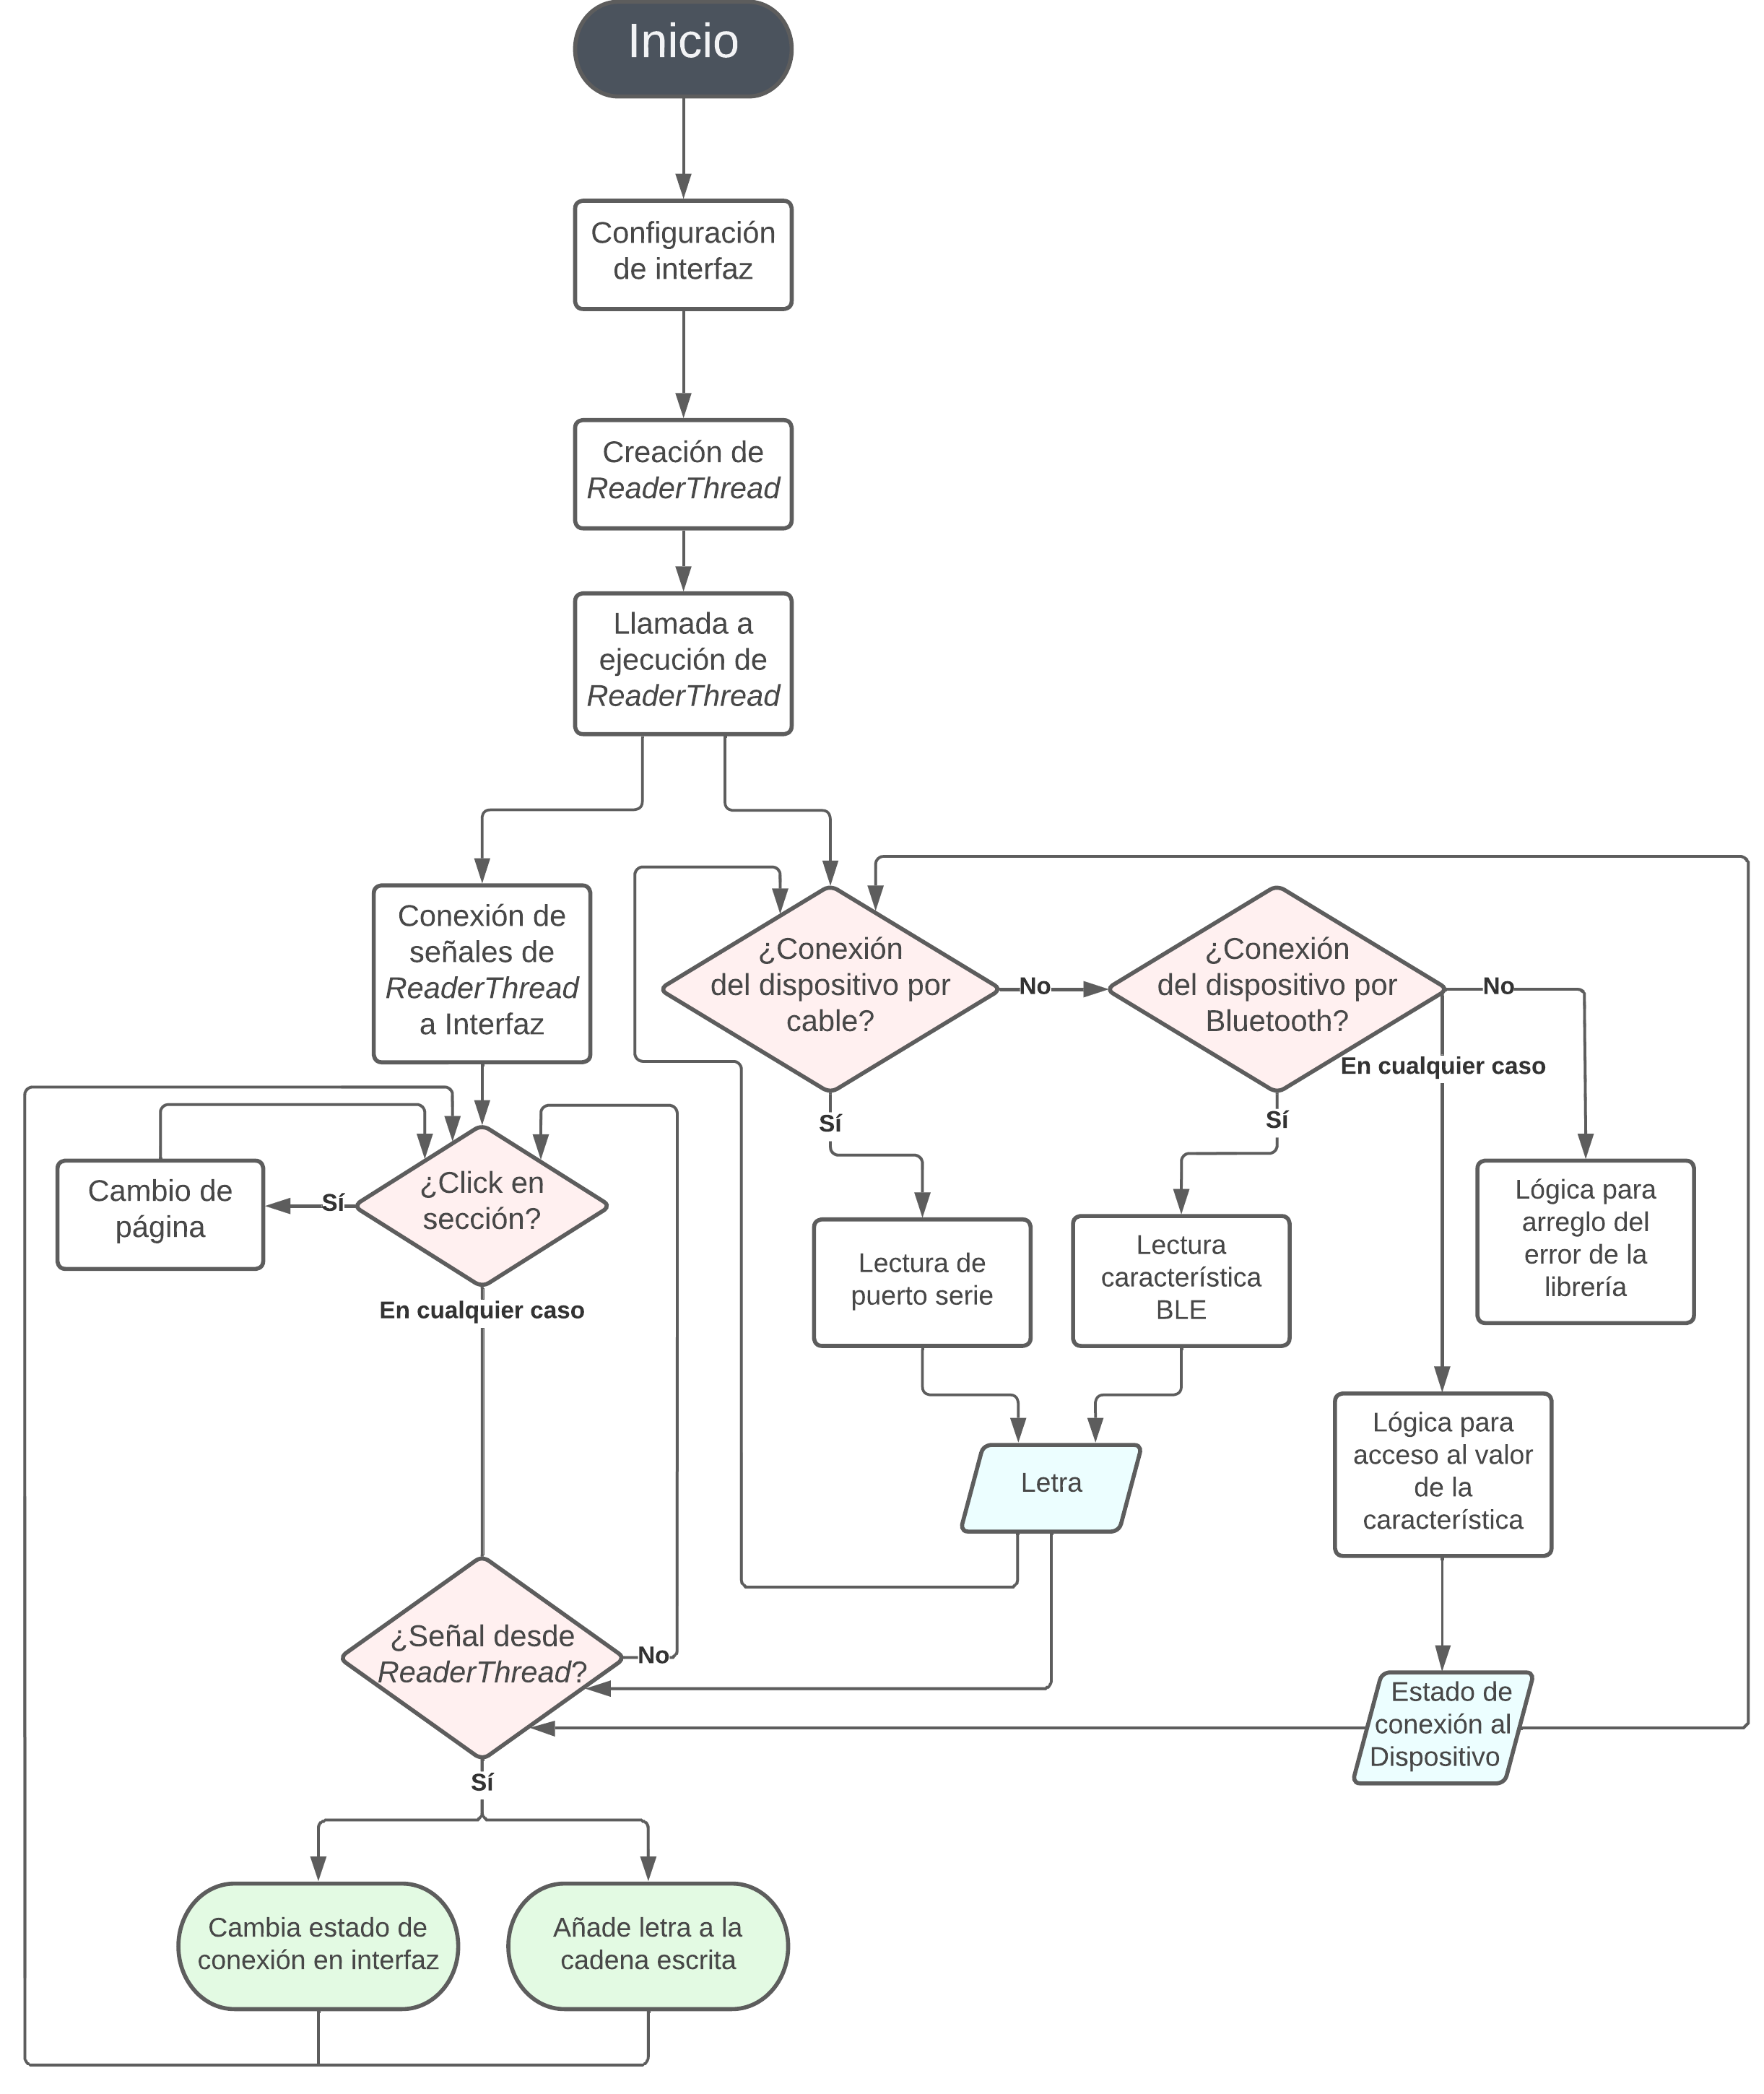
\includegraphics[width=1\textwidth]{capturas/DiagramaFlujoUI.png}\\[-0,20cm]
    \caption{Diagrama de flujo simplificado del \textit{UI}\label{diagFlujoQT}}
\end{figure}